% Set up document class and packages
\documentclass{article}
\usepackage{amsmath}
\usepackage{amssymb}
\usepackage{graphicx}
\usepackage{hyperref}
\usepackage{geometry}
\usepackage{amsfonts}
\DeclareMathOperator{\E}{\mathbb{E}}
\setcounter{secnumdepth}{0}

\geometry{a4paper, margin=1in}
\title{Endogenous Networks, Market Concentration, and Volatility}
\author{Ethan Nourbash}
\date{\today}

\begin{document}
\maketitle
\section{Introduction}
Herskovic et al 2020 find firm size dispersion positivley comoves with production variance and dispersion in variance. That is, the larger the dispersion in firm size. They explain the comovement using a network model of production.
\begin{center}
    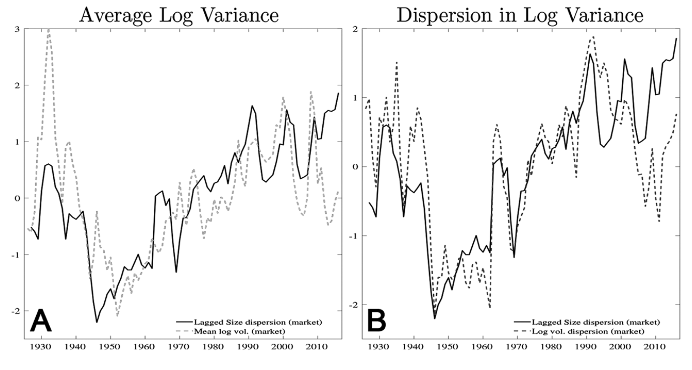
\includegraphics[width=0.8\textwidth]{figures/herskovic.png}
\end{center}
Variance and variance dispersion have risen alongside dispersion of firm size since the 1940s. 
The goal of this paper is to explain this trend by endogenizing production networks. \\
Model Features:
\begin{itemize}
    \item Consumer Risk Aversion
    \item Delivery uncertainty
    \item Heterogeneous productivity
    \item Minimum order size (or relation fixed cost)
    \item No Loops???
    \item Markets Clear ex-ante???
\end{itemize}
Risk aversion is adopted by the suppliers and makes them care about the volatility of their output. 
Differences in productivity creates firm size heterogeneity. 
Minimum order size makes optimal number of suppliers comove with firm size.
No loops (possibly) to make firm supplier decisions tractable and solve identification issue empirically.\\
Transactions occur ex-ante on expected quantities. Prices will capture volatility.
\\
The results are as follows:
\begin{itemize}
    \item An aggregate shock increases size of large firms, further increasing volatility.
    \item In certain situations, a shock to a large firm increases its size.
\end{itemize}
\section{Model}
\subsection{Real GDP}
\begin{align*}
    Y = \max_{\mathbf{c}} \E \mathcal{D}(\mathbf{c})
\end{align*}
$\mathcal{D}'>0$, $\mathcal{D}''<0$.\\
Subject to
\begin{align*}
    \sum_i^N p_i \E c_i = \sum_{i=1}^N \pi_i.
\end{align*}
\subsection{CRS firm production}
\begin{align*}
    y_i = A_i F(\mathbf{x_{i}}).
\end{align*}
Profits determined by marginal costs of inputs and fixed cost as a function of nonzero inputs. Networks are chosen before volatility is realized
\begin{align*}
    \pi_i = p_i \E y_i - \mathbf{p} \E \mathbf{x_{i}}
\end{align*}
subject to minimum \textit{expected} (due to uncertainty in delivery) order
\begin{align*}
    \E \mathbf{x_{i}} \geq c \mathbf{1}_N
\end{align*}
$c\geq 0$.\\
Productivity is log normal with idiosyncratic volatility with a common and firm-specific component
\begin{align*}
    \log A_i \sim N(0,\sigma + \sigma_i).
\end{align*}
Firms compete in bertrand competition.\\
Firms total volatility is a function of its own and that of its suppliers.\\
Orders are placed in expected values and recieved after $A_i$ is realized.
\subsection{Equilibrium}
An equilibrium is define when 1) markets clear 2) consumer is maximizing welfare given prices 3) firms maximize profits given other prices.

Issues with model:
\begin{itemize}
    \item Constraints on producer maximization problem lead to analytic difficulties.
    \item Relations determined simultaneuously (rather than loops) makes model complicated (or maybe impossible idk).
\end{itemize}
\end{document}

